\chapter{Resultados}

\par
Após realizar os experimentos para as ações PETR4.SA (Petrobrás), os modelos foram treinados, testados e avaliados em diferentes períodos, bem como suas previsões utilizadas em simulações de operações de trading. Os resultados dos 10 experimentos de cada período do CNN e LSTM foram submetidos à média e ao desvio padrão, e os demais testados para o ano de 2019 e 2020, posteriormente submetidos à média e desvio padrão também. Os gráficos de operações de trading abaixo são experimentos retirados dos testes feitos.


%---------------------------------------------------------------------------SUB

\subsection{\textbf{Previsões com CNN e Operações com Classifications Trading}}


%---------------FIGURE
\begin{figure}[hbt]
\centering
\caption{\label{figure:figura1}Previsões do CNN, seguido dos preços de fechamento reais e as operações de compra e venda, para 2020.}
  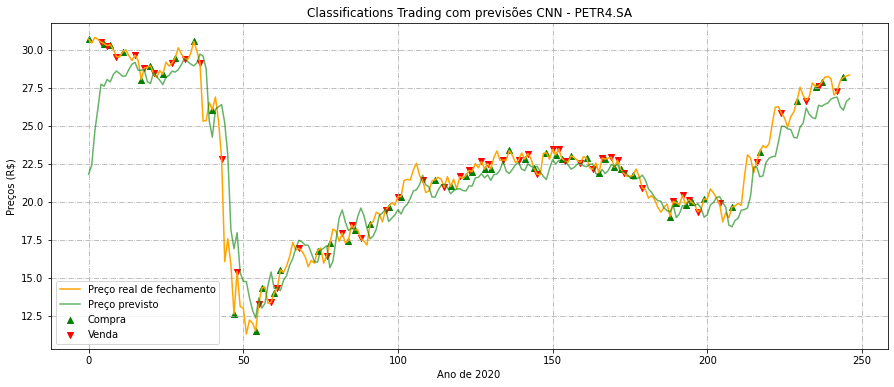
\includegraphics[scale=0.5]{figures/img18.png}
  Fonte: O autor do relatório.
\end{figure}


%---------------------------------------------------------------------------SUB

\subsection{\textbf{Previsões com LSTM e Operações com \textit{Classifications Trading}}}


%---------------FIGURE
\begin{figure}[H]
\centering
\caption{\label{figure:figura1}Previsões do LSTM, seguido dos preços de fechamento reais e as operações de compra e venda, para 2020.}
  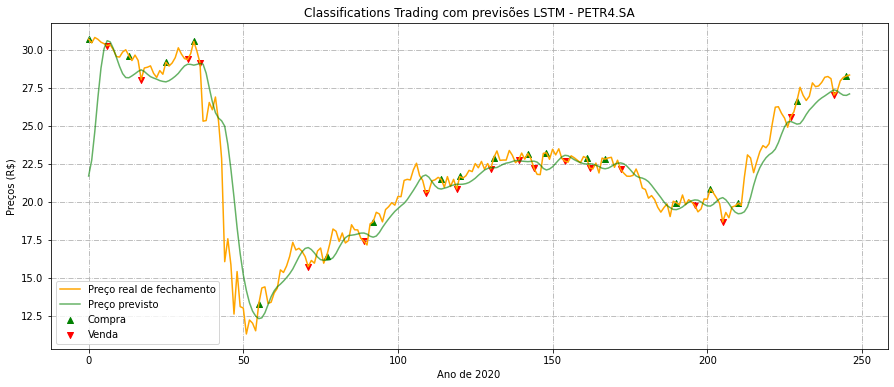
\includegraphics[scale=0.5]{figures/img19.png}
  Fonte: O autor do relatório.
\end{figure}

\subsection{Operações com \textit{Naive Trading}}


%---------------FIGURE
\begin{figure}[hbt]
\centering
\caption{\label{figure:figura1}Operações do algoritmo \textit{Naive Trading}, sem modelo, para o ano de 2020.}
  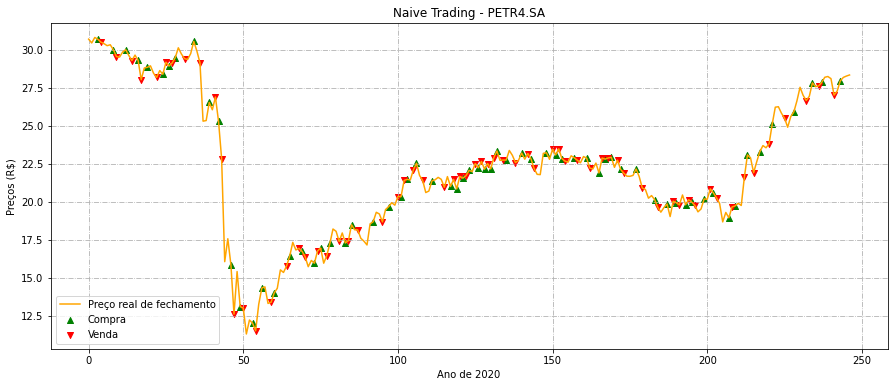
\includegraphics[scale=0.5]{figures/img13.png}
  Fonte: O autor do relatório.
\end{figure}

%---------------------------------------------------------------------------SUB

\subsection{\textbf{Médias dos resultados dos testes com as saídas numéricas}}


%---------------TABLE
\begin{table}[H]
\footnotesize
\centering
\caption{Médias dos resultados de todos os períodos dos testes feitos com cada técnica treinada, utilizando as saídas numéricas geradas pelo algoritmo e comparando os preços de fechamento com os preços reais observados.}
\begin{tabular}{ccccc}
\hline
\textbf{Técnica} & \textbf{Ação} & \textbf{Período} & \textbf{R2} & \textbf{MSE $({R\$})^{2}$} \\ \hline
CNN & PETR4.SA & Todos & 0.825285 & 1.736832 \\
LSTM & PETR4.SA & Todos & 0.923408 & 0.769675 \\
Modelo   Naive & PETR4.SA & Todos & 0.938442 & 0.475895 \\
AR & PETR4.SA & Todos & \textbf{0.955583} & \textbf{0.323019} \\ \hline
\end{tabular}
\center{Fonte: Autor do relatório.}
\end{table}

%---------------------------------------------------------------------------SUB

\subsection{\textbf{Médias dos resultados dos testes com as saídas categóricas}}


%---------------TABLE
\begin{table}[htp]
\footnotesize
\centering
\caption{Médias dos resultados de todos os períodos dos testes feitos com cada técnica, utilizando as classificações geradas pelo algoritmo e comparando os movimentos classificados como “alta” e “baixa” com os movimentos reais.}
\begin{tabular}{ccccccc}
\hline
\textbf{Técnica} & \textbf{Ação} & \textbf{Período} & \textbf{F1-Score} & \textbf{Acurácia} & \textbf{Precisão} & \textbf{Revocação} \\ \hline
CNN & PETR4.SA & Todos & \textbf{0.548317} & 0.527642 & 0.530769 & \textbf{0.567882} \\
LSTM & PETR4.SA & Todos & 0.480198 & 0.469783 & 0.47492 & 0.485627 \\
Modelo   Naive & PETR4.SA & Todos & 0.488195 & 0.477642 & 0.487201 & 0.489198 \\
AR & PETR4.SA & Todos & \textbf{0.595666} & \textbf{0.583006} & \textbf{0.588752} & \textbf{0.60276} \\ \hline
\end{tabular}
\center{Fonte: Autor do relatório.}
\end{table}


%---------------------------------------------------------------------------SUB
\subsection{\textbf{Médias dos resultados das operações}}


%---------------TABLE
\begin{table}[htp]
\scriptsize
\centering
\caption{Médias dos resultados de todos os períodos dos testes feitos com cada técnica combinada a um algoritmo de \textit{trading}.}
\begin{tabular}{cccccccc}
\hline
\textbf{Técnica} & \textbf{Ação} & \textbf{Período} & \textbf{ET} & \textbf{CI   (R\$)} & \textbf{CF   (R\$)} & \textbf{DC   (R\$)} & \textbf{RC} \\ \hline
CNN & PETR4.SA & Todos & Class.   T. & 100000.0 & 111,145.493793 & 11,145.493793 & \textbf{1.1114} \\
LSTM & PETR4.SA & Todos & Class.   T. & 100000.0 & 96,990.799319 & -3,009.200681 & 0.96990 \\
\textit{Modelo   Naive} & PETR4.SA & Todos & Class.   T. & 100000.0 & 80,634.992361 & -19,365.007639 & 0.80635 \\
AR & PETR4.SA & Todos & Class.   T. & 100000.0 & 127,029.992104 & 27,029.992104 & \textbf{1.2703} \\
Não   possui & PETR4.SA & Todos & \textit{Naive   Trading} & 100000.0 & 100,104.996681 & 104.996681 & 1.0010 \\
Não   possui & PETR4.SA & Todos & RMT & 100000.0 & 184,105.011702 & 84,105.011702 & \textbf{1.8410} \\ \hline
\end{tabular}
\center{Fonte: Autor do relatório.}
\end{table}


%---------------TABLE
\begin{table}[htp]
\footnotesize
\centering
\caption{Médias dos resultados de todos os períodos dos testes feitos com cada técnica combinada a um algoritmo de \textit{trading}.}
\begin{tabular}{cccccccc}
\hline
\textbf{Técnica} & \textbf{Ação} & \textbf{Período} & \textbf{ET} & \textbf{QOL} & \textbf{QOP} & \textbf{AOL} & \textbf{GMO   (R\$)} \\ \hline
CNN & PETR4.SA & Todos & Class.   T. & 33.5 & 22.7 & \textbf{0.595812} & 196.77536 \\
LSTM & PETR4.SA & Todos & Class.   T. & 19.5 & 33.0 & 0.372729 & -56.297246 \\
Modelo   \textit{Naive} & PETR4.SA & Todos & Class.   T. & 22.0 & 42.5 & 0.340909 & 18.793181 \\
AR & PETR4.SA & Todos & Class.   T. & 40.5 & 25.5 & \textbf{0.615278} & 408.08322 \\
Não   possui & PETR4.SA & Todos & \textit{Naive   Trading} & 31.5 & 32.0 & 0.496898 & 4.217068 \\
Não   possui & PETR4.SA & Todos & RMT & 64.0 & 0.0 & \textbf{1.0} & 1,311.769415 \\ \hline
\end{tabular}
\center{Fonte: Autor do relatório.}
\end{table}

\par
A figura abaixo compara algumas métricas utilizadas em teste, para os modelos CNN e \textit{Naive}; a última métrica representa a acurácia das operações com lucro (AOP), sendo uma métrica utilizada nas operações de trading de ambos os modelos. Essa comparação evidencia o desempenho da rede CNN diante de uma técnica simples de previsão em séries temporais.


%---------------FIGURE
\begin{figure}[hbt]
\centering
\caption{\label{figure:figura1}Comparação das métricas categóricas entre o CNN e o modelo \textit{Naive}, bem como a acurácia média das operações com lucro (última métrica).}
  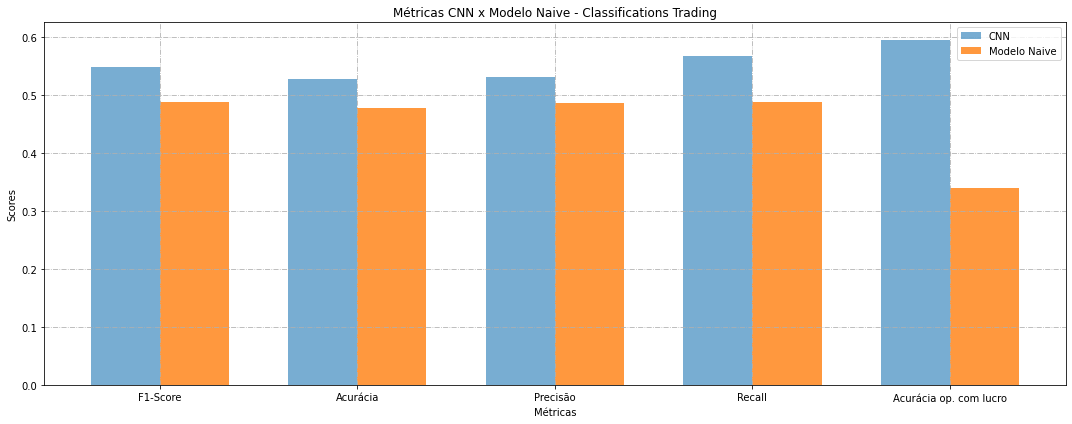
\includegraphics[scale=0.43]{figures/img15.png}
  Fonte: O autor do relatório.
\end{figure}